\documentclass[11pt]{article}
\usepackage{geometry}
\geometry{letterpaper,portrait,top=1in,bottom=1in,left=1in,right=1in}
\usepackage{parskip}
\usepackage{lscape}
\usepackage{graphicx}
\usepackage{hyperref}
\usepackage{setspace}
\usepackage{lineno}
\usepackage{tabularx}
\usepackage{amsmath}
\usepackage{pdfpages}
\usepackage{verbatim}
\usepackage{framed}
\usepackage{color}
\usepackage{soul}
\usepackage{natbib}
\usepackage{fancyvrb}
\usepackage{listings}

\setlength{\footskip}{3em}
\setlength{\headsep}{0em}

%Formatting for post-hoc text
\newcommand{\p}[1]{\textcolor{teal}{\textbf{#1}}}


\title{Performance Information and Voting Behavior in Burkina Faso's Municipal Elections: Separating the Effects of Information Content and Information Delivery\footnote{
This research is part of a long-term research partnership with Burkina Faso's \emph{Programme d'appui aux collectivit\'{e}s territoriales} (PACT). This research program, \emph{Recherche exp\'{e}rimentale sur la gouvernance locale au Burkina Faso} (REGLAB), involves a series of field experiments on municipal government performance and accountability. It has been supported by the World Bank and Yale University and through research grants from the Information Challenge Fund, the Knowledge for Change Program, i2i, and the World Bank's research support budget (RSB). We are grateful to Sidiki Soubeiga for local coordination and to Oulla Andr\'{e} Ouattara, Benjamin Sawadogo, Justin Yameogo, Idrissa Sor\'{e} and Serdar Yilmaz for their longstanding collaboration. The data collection for this study was funded by the EGAP Metaketa Initiative, implemented by Innovations for Poverty Action (IPA), and approved by Yale University's Human Subjects Committee (\#1405013896) and the Institutional Review Board at Innovations for Poverty Action (IPA) (\#14159). We are especially grateful to Alassane Koulibaly and Nicolas Orgeira for managing the fieldwork effort. We furthermore benefitted from excellent research assistance by Lars Nordgreen. Finally, we gratefully acknowledge advice, assistance and data received from Burkina Faso's Independent National Electoral Commission (CENI). 
}}
\author{Malte Lierl\footnote{Contact: malte.lierl@yale.edu. } \\ Marcus Holmlund\footnote{Contact: mholmlund@worldbank.org. }}
\date{October 4, 2017\\ *corrected version: May 11, 2018*}

\begin{document}

\maketitle

\doublespace

In this chapter, we report a field experiment in Burkina Faso, which aimed to isolate the effects of information content from other channels of influence through which an information intervention could affect voting behavior. The experiment was carried out in 38 rural municipalities, prior to the 2016 municipal elections. These 38 municipalities had been controlled by the same party for the past two electoral cycles, since the first nationwide municipal elections in 2006. In our experiment, we presented 741 randomly selected study participants with detailed information about their previous municipal government's performance along nine indicators of municipal service quality in the areas of health, primary education, water access, and civil services. These indicators reflected national standards for municipal services, i.e. widely accepted service delivery targets. Simultaneously, a control group of 752 study participants was presented merely with information about the indicators of municipal government performance, without any information on the actual performance of their previous municipal government. Thus, our experiment varied study participants' access to information about municipal government performance, but it held their knowledge of service delivery targets, as well as the method of information delivery, constant across the treatment and control conditions. 

Our research design allows us to make several unique contributions to the Metaketa initiative on information and accountability. First, we complement the other studies in the volume by focusing specifically on the effects of information content, in isolation from other aspects of information interventions. Often, political information interventions do much more than just providing voters with information. For example, they prime or educate voters about specific aspects of incumbent performance \citep{Banerjee2010,Lieberman2014}, convey normative messages about what constitutes good performance \citep{Chong2013}, suggest metrics by which voters can compare different candidates \citep{Humphreys2012a}, and involve media consumption \citep{Reinikka2005,Aker2017} or direct social interaction with the individuals who provide the information. In most information interventions, these treatments are bundled together. We aim to disentangle the effects of information content from how the information is delivered, by comparing two experimental conditions that only differed with respect to the availability of factual information about the performance of the incumbent government, holding the method of information delivery constant. In this respect, our experiment resembles \citet{Gottlieb2016}, which varies whether or not a civic education course included information about local government performance. It differs from \citet{Gottlieb2016} in that our study is carried out at the individual level, focusing on individual-level heterogeneity in the effect of information access on pro-incumbent voting. 

A second unique aspect of this study is its results-blind approach to data analysis. In addition to elaborating our original motivations for the study in a pre-analysis plan, we carried out a first pass of data analysis on a blinded data set. In the blinded data set, any variables that would have allowed us to infer the experimental condition an individual was assigned to were obscured. However, the total number of treated and control units and the unconditional distribution of outcome variables and covariates was preserved, by randomly permuting the treatment assignment variable in the data set. Blind analysis prevents researchers' knowledge of experimental results from consciously or unconsciously influencing their choice of analytical methods, which can cause them to over-interpret results. While blind analysis has become a standard procedure in experimental physics \citep{Klein2005}, its adoption in the social sciences is limited (see \citet{Humphreys2013} for a notable exception). Compared to a pre-specified analysis plan (a practice that has been criticized for being error-prone and leading to ``robotic'' data analysis \citep{Gelman2013}), a results-blind analysis allows for methodological choices in data processing and data analysis that are informed by the actual data and by descriptive inferences about the study population. We documented this blinded analysis by submitting a full, results-blind report to the EGAP experimental design registry,\footnote{\url{http://egap.org/file/2154/download?token=Fe0o2HOiBjiUTz5HUR6IxZJSu9epz0RMNV18-IeSoG0}} and then replicating this results-blind analysis with the final, non-blind dataset.\footnote{\url{http://egap.org/file/2388/download?token=hzbpFKTGCTjreLgFnttdrSQh9-8jPWU6PcMl3ijLTDA}} 

This chapter draws on material from \citep{LierlHolmlundAmbiguity}, which reports our study in greater detail. 

\section{Local Government Performance and Electoral Accountability in Burkina Faso}

Burkina Faso is a low-income, land-locked multi-ethnic West African country of about 18 million inhabitants, covering three climate zones, from the hot, arid Sahel zone in the north, to a tropical savanna climate in the country's south. Like many other low-income countries, Burkina Faso adopted a decentralized system of local governance in the early 2000s. Since the first nationwide municipal elections in 2006, elected municipal governments have played an important role in the provision of local-level public services in Burkina Faso. Municipal governments provide inputs and services that are critical for the ability of primary schools and health centers to serve the population. Additionally, they are responsible for the maintenance of water points, which are one of the most important local infrastructures in Burkina Faso's hot and semi-arid climate. Municipal governments also provide important administrative services, such as the civil registry. 

Even though municipalities have only partial responsibility for the performance of certain public services, such as schools and health centers, their failure to provide the necessary inputs and authorizations to service providers is more often than not a limiting constraint on the overall quality of these services. For example, municipal governments in Burkina Faso are responsible for procuring gas bottles for health clinics, which are needed to operate their refrigerators. If municipalities fail to replenish the gas stock on time, vaccines and medications will spoil and health centers are unable to treat their patients. Gas stock-outs and similar service failures are widespread and can have devastating externalities for local health, education and development outcomes. The frequency of such failures is indicative of a fundamental problem in local government accountability: Municipal administrators usually have few consequences to fear if they do not live up to their stated responsibilities  \citep{Mahieu2010}. This is suggestive of inherent limitations of electoral and bureaucratic accountability at the local level.  

\subsection{Local-level electoral accountability}

In the past, one of the major obstacles to electoral accountability was a lack of political competition. During the first two municipal elections in 2006 and 2012, the national party in power, the \emph{Congr\`{e}s pour le d\'{e}veloppement et le progr\`{e}s} (CDP), won the vast majority of municipal council seats. In 2006, the CDP commanded 12,854 out of 17,786 municipal council seats. In 2012, 12,340 out of 18,552 council seats. Municipal councils elect the mayors, who in turn head the municipal governments. Mayors are elected without term limits. Municipal councils, in turn, are elected by the residents of the municipality in the municipal elections. On the municipal council, every village of the municipality is represented by two delegates. In communes with fewer than ten villages, the number of council delegates is adjusted upwards in proportion to population size, for a minimum council size of twenty. Municipal councilors are elected by party lists. This means that voters choose between parties, not between individual candidates. Ballots are unique by municipality, but not by village. Mayors are typically from the party that wins the most municipal council seats. 

In 2014, the CDP's stronghold on power crumbled. On October 31, 2014, former president Blaise Compaor\'{e} was ousted in a popular uprising, reacting to his attempt to circumvent his term limit by manipulating the constitution. The CDP government was replaced by a military government that eventually agreed to form a joint military-civilian transition government under a civilian interim president, but with military control over key cabinet positions. The transition government adopted a roadmap towards democratic multi-party elections. However, the plan to hold elections was put in jeopardy by a violent coup d\'{e}tat by the presidential guard in September 2015, an elite special force loyal to the former president Blaise Compaor\'{e}. The junta encountered massive resistance from civil society. After one week, the national army intervened against the presidential guard, forcing the junta to surrender. The transitional government was reinstalled and peaceful national elections were held in November 2015, the results of which were recognized by all parties. Under the new national government, led by the majority-winning \emph{Mouvement pour le progr\`{e}s} (MPP), transitional municipal elections were announced for May 2016. The May 2016 municipal elections marked the end of Burkina Faso's political transition. Figure \ref{FigTimeline} visualizes this timeline. 

In the wake of the popular uprising, the civil-military transition government dismissed all elected municipal governments in December 2014 and replaced them by non-partisan, externally appointed special delegations. These special delegations were mandated to carry out the institutional responsibilities of the previous elected municipal councils and mayors, operating within the same legal and institutional frameworks. However, members of the special delegations were not eligible for candidacy in the 2016 municipal elections. The special delegations merely acted as interim caretakers, to fill the void created by the dismissal of the incumbent municipal governments. Thus, in the 2016 municipal elections, the previous incumbent parties competed with the newly strengthened opposition parties, giving most voters greater freedom of choice than ever before. 

\begin{figure}
\begin{center}
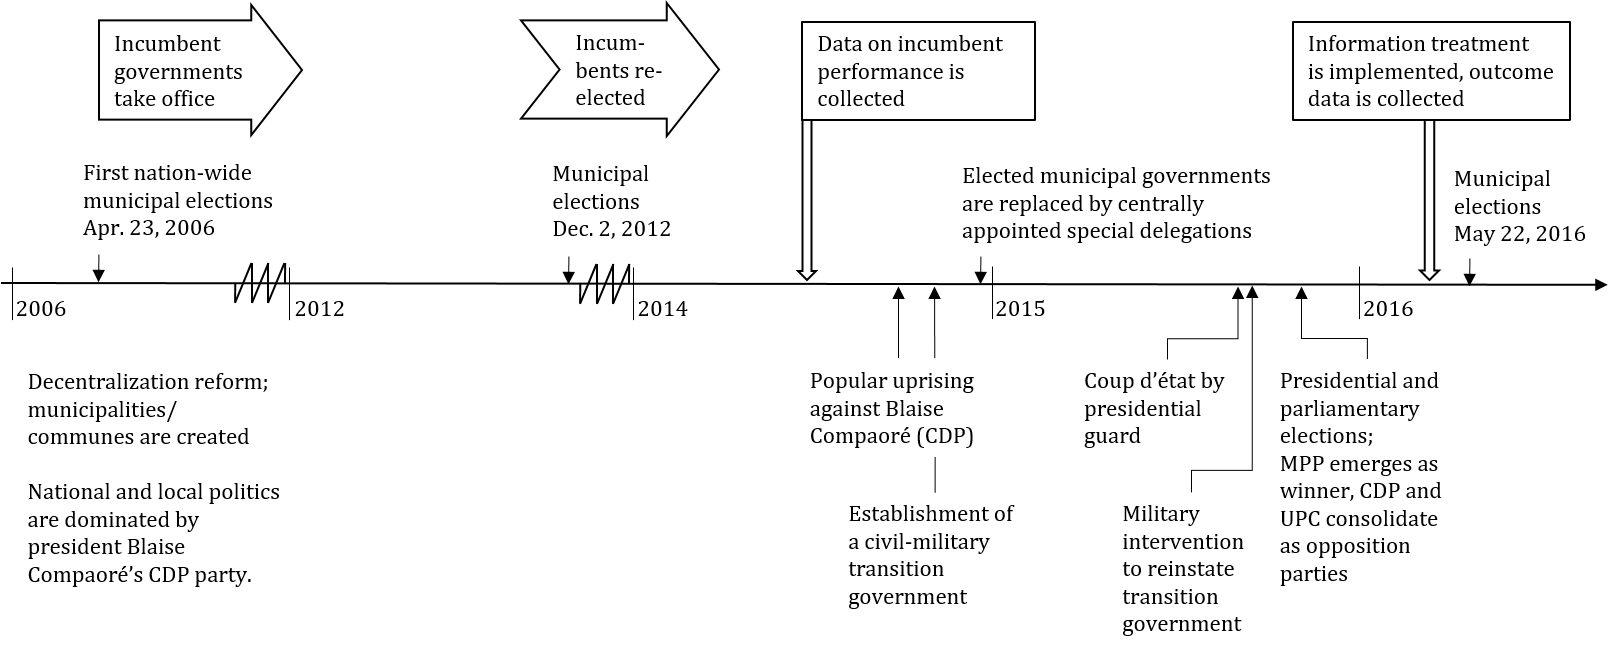
\includegraphics[width=\textwidth]{Figures/BF_Timeline.png}
\end{center}
\caption{Timeline. }
\label{FigTimeline}
\end{figure}

\subsection{Distinctive features of the Burkina Faso case}

The municipal elections in Burkina Faso differ in several respects from other cases in this volume. First, voters' access to information is particularly limited. Burkina Faso has one of the lowest levels of formal education in the world. While adult literacy rates have been increasing steadily in recent years, they remain extremely low at 38 percent\footnote{Source: Database query at http://data.worldbank.org [2017-02-19]. }. In our study sample, only 15 percent of respondents report knowing how to read and only 14 percent report having completed any kind of formal education. The low levels of literacy and formal education create a context in which citizens' access to political information is naturally restricted. This means that written media have only marginal importance as sources of political information, whereas face-to-face communication and radio programs are potentially more important than in other contexts. %[add information from 2015 survey on the relative importance of different information channels?]

Second, conducting a political information experiment in a multi-ethnic population with very limited access to formal education involved particular challenges. Perhaps the greatest challenge was to present information in a way that is accessible to illiterate citizens with different linguistic backgrounds. Additionally, the information had to be accompanied by an explanation of its relevance, in terms of its implications for the lives of ordinary citizens. Therefore, any form of information provision had to be accompanied by substantial additional explanation and interaction. This created a particular research design challenge: Should the experiment evaluate the impact of a bundled treatment (an information campaign that includes elements of civic education, interpersonal interaction, etc.), or should it try to isolate the causal effect of the information content, while holding all other elements of the information intervention constant? 

Several other studies in this volume pursue the first-mentioned approach, evaluating the aggregate electoral impact of a bundled information intervention, for example of the public video screening of candidate statements (Platas and Raffler in this volume), or the distribution of print media by an advocacy NGO (Arias et al. in this volume). These approaches have the advantage of generating evidence about a realistic social intervention (especially if implemented in collaboration with local NGOs or other potential scale-up partners). In contrast to these other studies, we opted for the second approach, pursuing a highly controlled individual-level information experiment on a relatively small sample of voters. We hold all explanations and interactive procedures constant between the treatment and control groups and only vary the availability of actual information content about the performance of the incumbent municipal government. This approach has the advantage of isolating the effects of information access from other mechanisms, making causal attribution unambiguous and hence making it possible to test theoretical hypotheses at a higher level of abstraction. In part, this decision was due to the specific challenges, including ethical questions, of carrying out a large-scale voter information campaign in Burkina Faso's fragile political environment -- a research context that substantially differed from the other studies in this volume. Additionally, however, our highly controlled experiment complements this book's research agenda by shedding light on the most crucial element of the causal chain that links information interventions to changes in electoral behavior: the information content itself. 

There are several additional respects in which our experiment contrasts with the other studies in this volume. 
First, our information treatment was targeted at the individual level and therefore relatively limited in scope, covering merely 758 individuals across 39 municipalities. We had no reason to expect that local politicians would react to the provision of information to voters, nor did we observe any such reactions. In contrast to interventions with much broader coverage, such as Chauchard and Sircar (this volume) and Arias et al. (this volume), there was no indication that ``[p]oliticians mount[ed] campaigns to respond to negative information'' spread through our information treatment (Hypothesis H5 in the meta-analysis plan), or that they reacted to positive information in any way. We also did not expect any measurable impact on aggregate election outcomes. For this reason, we focus our analysis on individual voting behavior. 

Second, our study concerns the electoral accountability of political parties in a closed-list proportional representation system, rather than of individual politicians in single-member districts. In a closed-list system, voters cannot hold individual candidates accountable, but have to choose between party lists. Mayors are indirectly elected by municipal council majority, and there are no officially designated mayoral candidates prior to the constitutive session of the newly elected municipal councils (although, in case of the incumbent party, it is usually obvious to voters that the incumbent mayor or her/his chosen successor will seek re-election by the council if the incumbent party wins the election). For these reasons, information about individual list candidates is potentially less relevant for voters than information about the overall performance of the incumbent government. 
  
Since information about municipal government performance is not easily attributable to individual candidates, but rather to incumbent parties as a whole, we do not analyze the impacts of performance information on perceptions of candidate integrity and candidate effort (Hypotheses H3 and H4 in the meta-analysis plan by \citet{MetaPAP}). These outcomes are politician-specific and cannot easily be generalized to parties as a whole. Furthermore, political parties in Burkina Faso are cross-ethnic and do not usually campaign on platforms that emphasize special interests of particular ethnic groups. Therefore, it is not directly possible to identify whether a party is ``co-ethnic'' or ``non-co-ethnic'' from a voter's perspective. This limits our ability to evaluate Hypothesis H6 in the meta-analysis plan, that ``[i]nformation effects are more positive for voters that do not share ethnic identities'' \citep[5]{MetaPAP}. 

\section{Experimental Design and Data}

\subsection{Treatment and control conditions}

Our experiment was designed to hold all aspects of the information intervention constant between the treatment and control conditions, except for the availability of actual information content. To achieve this, we provided study participants in both the treatment and control groups with identical and detailed explanations of a municipal governments' most essential inputs to local public services in the areas of primary education, health care, water, sanitation and civil services, as well as their relevance for citizens' everyday lives. We also provided study participants with information about national standards for municipal service delivery in these areas. For most study participants, these benchmarks were new information. Additionally, we confronted study participants in the treatment and control groups with an identical set of survey questions to measure their prior beliefs about their municipal government's performance, their assessment of different electoral candidates and their electoral participation.  We therefore consider our control condition a ``placebo" or ``baseline" treatment that is equally applied to members of the treatment and control groups. 

Relative to this control condition, our study evaluates the effect of individual-level access to factual information content regarding the performance study participants' previous (and  temporarily suspended) incumbent municipal government. These previously elected incumbent governments were competing for re-election in the May 2016 municipal elections. Since the special delegations that temporarily replaced them between January 2015 and May 2016 were non-partisan, technocratic and barred from candidacy in the municipal elections, we consider the party that had won the previous municipal elections in 2012 to be the incumbent. 

It is important to emphasize that the performance information we presented to study participants in the treatment group is unambiguously attributable to the previous incumbent municipal government, rather than to the performance of the interim special delegation. It is based on data we collected in 2014, prior to the popular uprising and prior to the dismissal of the elected municipal governments. Moreover, the incumbent parties in our study had been in power for an uninterrupted period of eight years. Given that elected municipal governments were only created in 2006, this means that incumbent government's performance record cannot have been influenced by a predecessor government. 

Assignment to the treatment and control conditions was block-randomized at the individual level with equal numbers of treatment and control units per village. To eliminate spillover effects within villages, the performance information in the treatment condition, as well as the information about performance benchmarks in both the treatment and control conditions, were provided to study participants in a one-on-one setting, through a flashcard presentation by our surveyors. Our outcomes of interest, including intended vote choice and propensity to turn out to vote, were measured immediately afterwards through a polling station simulation and a set of survey questions. 

In what follows, we describe in greater detail the type of information study participants in the treatment and control conditions were given, as well as the procedure for delivering this information. 

\subsection{Information content}

Our information about the performance of the previous incumbent municipal governments is based on a municipal government performance survey we carried out in 2014. Based on the survey data, we calculated nine indicators of municipal service delivery performance in the areas of primary education, primary health care, water, sanitation, and administrative services: 
\begin{enumerate}
\item The difference between primary school completion rates in the municipality and the national average;
\item The average delay in the provision of school supplies at the beginning of the school year;
\item The proportion of births taking place at a health facility;
\item The proportion newborns having received the full set of recommended vaccines;
\item The proportion of primary healthcare facilities receiving a sufficient supply of natural gas each month (for refrigeration);
\item The proportion of residents with access to a functioning source of clean water, defined according to the national norm (a source located within a distance of 1000m or less that is shared by no more than 300 people);
\item The proportion of primary schools with a functioning source of clean water;
\item The proportion of primary schools with functioning latrines;
\item The proportion of newborns for whom a birth certificate was issued.
\end{enumerate}

This combination of performance indicators was selected to satisfy six criteria. Each individual indicator is (1) tied to activities within the legal and practical purview of municipal governments, (2) substantively significant for citizens' quality of life, (3) measurable in quantitative and objective terms, (4) based on information that is already available or can be collected at low cost, (5) comparable across municipalities and over time, (6) consistently relevant across Burkina Faso's socially and ecologically diverse regions, and (7) low-dimensional and understandable without technical training. 

The selection and validation of the performance indicators was a year-long iterative process that involved close exchange with our government partner, the Territorial Collectivities Support Program (\emph{Programme d'appui aux collectivit\'{e}s territoriales}, or PACT) of the Ministry of Territorial Administration and Decentralization (MATD), the review of primary documents, field visits of municipal administrations and service providers in the Sahel and Plateau Central regions, and consultations with approximately forty mayors as well as with technical and administrative staff at the municipality levels. Additional comments were received from the Ministry of Health, Ministry of Education, the Ministry of Water, several national NGOs, as well as the National Land Management Program (PNGT). The relevant statistical directorates were consulted at the national, regional, and district levels on the availability and quality of data and site visits were carried out to understand the availability and quality of primary records at health facilities, health districts, school districts and municipal administrations. The end result is a set of indicators for which clearly defined national performance standards exist and that are readily acknowledged by municipal officials to be within their scope of responsibility. 

\subsection{Information delivery}

%\emph{Control condition: information on municipal service delivery norms}

Study participants in both conditions were provided with information about widely-accepted benchmarks for municipal service quality. Study participants were informed that: 
\begin{quote}
``For the different responsibilities of municipal governments, for example with respect to primary education, health, water supply and sanitation and administrative services, there are certain national standards every municipal government should fulfill. But not all municipal governments perform equally well at attaining these standards. I am now going to show you some images that depict several important responsibilities of municipal governments. I will also explain to you why these responsibilities of municipal governments are important. At the end, I am going to ask you how well, in your opinion, the previous elected municipal government in your commune performed at fulfilling those responsibilities.''
\end{quote}
Subsequently, study participants received an interactive presentation of each of the nine performance indicators, using illustrated flashcards. These illustrations were produced by an experienced Burkinab\'{e} illustrator who had previously visualized information for illiterate populations. The illustrations were repeatedly pilot-tested on both illiterate and literate citizens and refined until they were fully and easily understood. The flashcards contained two contrasting images that illustrated the respective norm and its importance. 
The two images differed only with respect to the presence or absence of a municipal government input. For example, one image would show a child using a latrine on the school yard, whereas in the other image the latrine was lacking and the same child would defecate in the open in the same place of the school yard (Figure \ref{FigFlashcards}). Respondents were asked to identify the difference between the two pictures. 

\begin{figure}
\begin{tabularx}{\textwidth}{|l l|}
\hline
&\\
\includegraphics[width=0.47\textwidth]{Figures/BF_Latrine-1bw.png}
&\includegraphics[width=0.47\textwidth]{Figures/BF_Latrine-0bw.png}\\
&\\
\hline
\multicolumn{2}{X}{ }\\
\hline
&\\

\includegraphics[width=0.47\textwidth]{Figures/BF_Water-1bw.png}
&
\includegraphics[width=0.47\textwidth]{Figures/BF_Water-0bw.png}\\
&\\
\hline
\end{tabularx}
\caption{Flashcard illustrations of municipal performance indicators. Top: Provision of school latrines. Bottom: Provision/maintenance of water points. }
\label{FigFlashcards}
\end{figure}

After being asked to explain the message of each flashcard to the surveyor, study participants were read a brief description of the importance of this particular aspect of municipal performance for citizens' lives. For example, in the case of school latrines, the following explanation was given: 
\begin{quote}
``Municipal governments have to ensure that all primary schools have a functioning latrine for each class. A functioning latrine provides a safe place for schoolchildren to urinate and defecate. Access to a functioning latrine is important, because otherwise the schoolchildren lack a safe place where they can keep good hygiene and preserve their dignity. If the children do not have access to functional latrines at school, this could increase the spread of epidemic diseases and discourage young girls from attending school. Certain diseases, such as diarrhea or cholera, can spread easily if children do not use proper sanitation.''
\end{quote}
In the case of functioning water points, it was explained that: 
\begin{quote}
``Municipal governments have to ensure that all people have access to a functioning source of potable water that is at most 1 km away and for no more than 300 people.  A borehole provides potable water from the ground. Access to potable water is important, because otherwise people will get sick. Also, if people do not have access to clean water close to their homes, they will spend a lot time fetching water, instead of using this time for income-generating activities or to send young girls to school.''
\end{quote} 
Analogous descriptions were provided for each of the nine indicators, with the full process (flashcards, interactive questions and explanations) taking approximately ten minutes. The original French scripts were repeatedly translated into six vernacular languages and back-translated into French, until we arrived at a version that was equally well understood in each of the six languages. While the English translation above appears slightly awkward and wordy, this is owed to the fact that it closely follows the version that worked best in Moor\'{e} and the other vernacular languages. 

During the presentation of the flashcard illustrations, the surveyors recorded, without the respondents' knowledge, whether or not the respondent had correctly understood the meaning of the indicator just by comparing the two illustrations, prior to the explanation of the indicator. The data show that over 70 percent of respondents correctly understood the illustrations of at least eight of the nine performance indicators. The primary source of comprehension problems was the indicator concerning the average delay in the delivery of school supplies. This was arguably the most complex indicator (involving averages across schools) and also the most challenging indicator to illustrate (because delay is not the same as absence). It was understood by only 53 percent of respondents (Table \ref{TableComprehension}). 

Following the presentation of the nine indicators, surveyors recorded study participants' beliefs about the performance of their previous incumbent municipal government (before the regime change in October 2014) along these dimensions of service delivery. Study participants were asked about their beliefs in two ways. First, in terms of five broad descriptive categories. Second in terms of their municipality's rank within of their region (the total number of municipalities in the region was provided in the question prompt). Study participants were also asked about their certainty with respect to each of these assessments, and about their assessment of the level of effort of their previous elected mayor compared to that of most other mayors in the region. This concluded the ``control'' condition.

\subsubsection*{Experimental variation: information on municipal service delivery norms with and without performance information}

In addition to the presentation of the performance indicators, participants assigned to the treatment group received information about their previous incumbent municipal government's actual performance along these indicators. This information was again delivered through flash cards, which contained the municipality's name, written information (that was read aloud by the surveyor), as well as a simple bar chart illustrating the indicator value (Figure \ref{FigFlashcardInfo}).  

\begin{figure}
\begin{center}
\begin{tabularx}{0.8\textwidth}{|X|}
\hline
\vspace{0.1em}
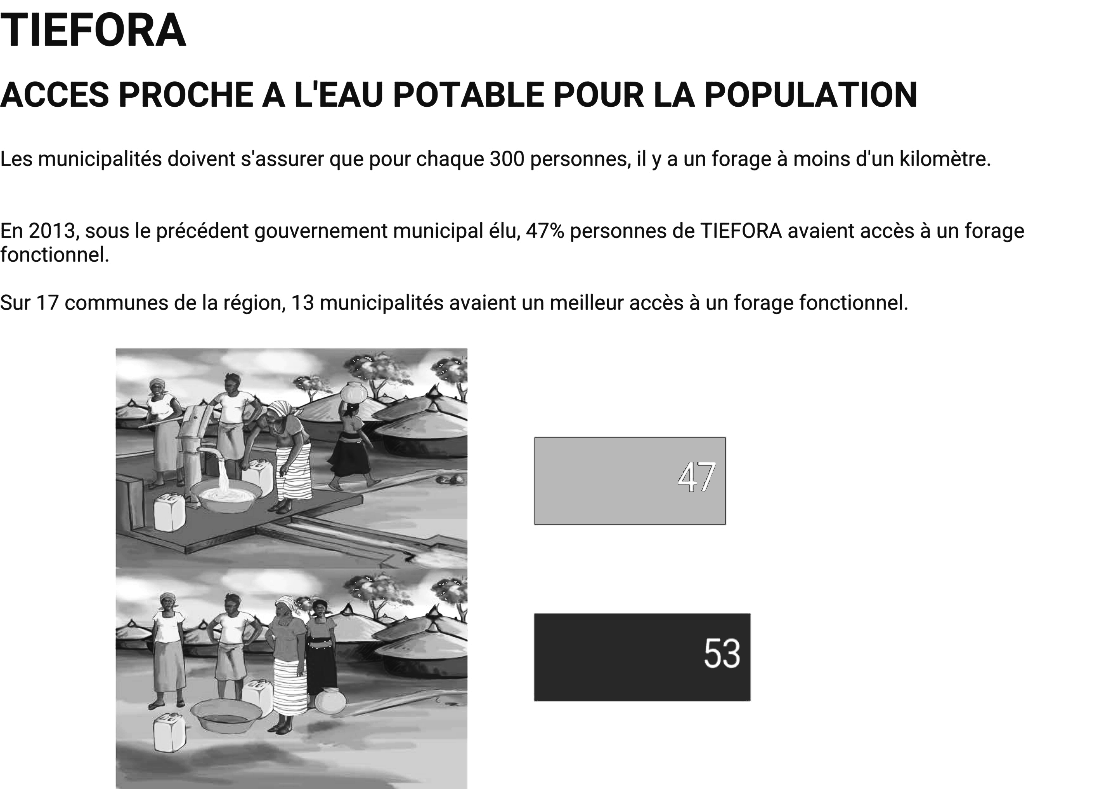
\includegraphics[width=0.76\textwidth]{Figures/BF_Water-Infobw.png}\\
\hline
\end{tabularx}
\end{center}

\caption{Flashcard presentation of the municipal performance information (municipality of Tiefora). The text reads: ``Municipalities must ensure that for every 300 people, there is a borehole available within 1 kilometer. In 2013, under the previous elected municipal government, 47\% of persons in Tiefora had access to a functioning borehole. Out of 17 municipalities in the region, 13 municipalities had better access to functioning boreholes.''}
\label{FigFlashcardInfo}
\end{figure}

The information flashcards were accompanied by a brief explanation, read aloud by the surveyor: 
\begin{quote}
Now, I would like to tell you about the availability of latrines at primary school in the municipality of [MUNICIPALITY] in 2013, under the previous elected municipal government that was controlled by the [INCUMBENT PARTY]. In this graphic, the LENGTH of the green bar indicates the proportion of schools that have functional latrines for each class and the length of the red bar indicates the proportion of schools without functional latrines for each class. In 2013, [$x$] out of every 100 primary schools in [MUNICIPALITY] had access to functional latrines for each class. This means that in [$1-x$] percent of the schools, the previous elected municipal government had not provided functional latrines for each class.
\end{quote}
The flashcards and explanations were given for all nine indicators as well as for the overall performance rating of the municipality. This process took approximately ten minutes. Following the information treatment, surveyors and study participants were asked a series of questions to measure attentiveness to, interest in, and comprehension of the information treatment. 

\subsection{Understanding of the information content}

We asked the interviewers administering the information treatment to subjectively evaluate each study participant's attention to the information treatment, on a scale from 1 (completely bored) to 10 (extremely attentive). On 844 data points (including five additional municipalities in which the incumbent party was no longer running for re-election), the average score was 6.79, with standard deviation 2.19, and 4 missing values. This is consistent with study participants' self-reported interest in the information treatment. After being informed about the information source, study participants were asked how credible they found the information. 83.5 percent of respondents described the information as ``credible'', another 13.2 percent as ``probably credible''. Moreover, study participants were asked about the pertinence of the information (``If you wanted to explain to your friends how well the previous elected municipal government performed at fulfilling its responsibilities, how useful would this information be?''). 83.8 percent claimed to find the information ``very useful; more useful than any other information'', another 12.9 percent described it as ``useful, but other information would have been more useful''. Finally, study participants were asked if, in all honesty, they found the information interesting or boring. 74.5 percent described the information treatment as ``very interesting'', another 22.4 percent as ``somewhat interesting'', and only 1.2 percent described it as ``somewhat boring'' or ``very boring''. Thus, at least according to study participants' self-reports, the information treatment was widely perceived as credible, pertinent and interesting. 

Furthermore, despite the complexity of the performance information, a majority of study participants found it understandable. 51.7 percent found it ``easy to understand'', 27.5 percent found it ``understandable, but complicated'', while 20.8 percent found it ``very difficult to understand''. Study participants' initial understanding of the performance information was verified through comprehension checks that were conducted after information treatment. For example, study participants were asked: ``How well did your previous elected municipal government perform with respect to the proportion of schools with a functioning water source, in comparison to other municipal governments in your region? Better, about the same, or worse?'' Depending on their response, study participants were then told if their answer was correct or incorrect. If study participants answered incorrectly or indicated that they did not know the answer, they were given the correct answer to ensure that they subsequently internalized the information. Table 2 summarizes the initial comprehension checks. Depending on the indicator, between between 59 and 63 percent of respondents were able to correctly recall the information. 

\begin{table}

    \begin{center}
    \begin{tabular}{l c | c }
    \hline
    Indicator&\multicolumn{2}{c}{Proportion of study participants}\\
    &correctly interpreting&correctly recalling\\
    &illustrations without&performance information\\
    &verbal explanation&at first attempt\\
    \hline
    School Water Sources&0.74&0.61\\
    School Latrines&0.84&0.63\\
    School Supplies&0.53&0.59\\
    CEP Admission&0.76&0.58\\
    Functioning Water Points&0.9&0.58\\
    CSPS Gas Stockouts&0.73&0.6\\
    Infant Vaccination Rates&0.87&0.6\\
    Assisted Deliveries&0.76&0.62\\
    Birth Certificates&0.76&0.62\\
    Observations  &1493&741\\
    \hline\hline
    \end{tabular}
    \end{center}
    

\caption{Intuitive comprehension of the graphic illustrations of performance indicators (left) and correct recall of performance information (right). }
\label{TableComprehension}
\end{table}

\subsection{Study population}

The population of interest for our study are voting-age adults, i.e. residents of a municipality who are eligible to vote (i.e. aged 18 and above) and unlikely to suffer from mobility constraints that might impede them from voting or otherwise exercising their rights to participate in local governance processes. This was proxied by sampling individuals who were between 18 and 70 of age in a census of adult village residents that was carried out in 2014. Table \ref{TableDescriptiveStats} describes this study population. 

\begin{table}

    \begin{center}
    \begin{tabular}{l c c c}
    \hline
    &Treatment Mean&Control Mean&P-value Difference\\
    \hline
    Age (years)&39.43&39&0.55\\
    Female&0.5604&0.57&0.71\\
    Years of education&0.68&0.86&0.11\\
    Literate&0.133&0.15&0.34\\
    Voted in 2012&0.63087&0.63&0.97\\
    Voted for incumbent in 2012&0.5456&0.54&0.83\\
    Relative living conditions $[-2,2]$&-0.0283&0.0037&0.53\\
    \hline\hline
    \end{tabular}
    \end{center}
    \caption{Demographics of the study population and tests of balance between treatment and control group. }
    

\label{TableDescriptiveStats}
\end{table}

\subsection{Study sites and sampling procedure} 

We carried out our research in six of Burkina Faso's thirteen regions, covering each of the country's main cultural and geographic zones, from North to South: Sahel, Centre-Nord, Plateau Central, Centre-Est, Centre-Sud, and Cascades (Figure \ref{FigMap}). Within these six regions, our study covered a total of 39 municipalities that satisfied the following inclusion criteria: (1) They were part of a random sample of 58 rural municipalities in which we carried out an experimental ``citizen observer'' intervention through which randomly sampled voting-age citizens were invited to observe meetings of the special delegations \citep{CitizenObserverPAP}. (2) They were governed by the same incumbent party since the first municipal elections in 2006, i.e. the incumbent party was re-elected in 2012. Out of the 44 municipalities that satisfied these inclusion criteria, 40 were controlled by the CDP, three by the CFD-B, and one by the ADF/RDA. In 31 of these 44 municipalities, the incumbent party was running again in the 2016 municipal elections. In eight additional municipalities, the incumbent party had dissolved or merged into a different party, and the incumbent mayor was running for re-election that party's name.\footnote{Of the three CFD-B mayors in the sample, two were now running for the UPC and one for the NTD. In four municipalities where the CDP had dissolved locally, two mayors were running for the NAFA, one for the NTD, and one for PAREN.}  In those cases, we treat the incumbent mayor's party in the 2016 elections as the incumbent party. In one of these cases, the incumbent CDP government was running unopposed under the MPP's name. We exclude this municipality from the study and limit our analysis to the 38 municipalities in which the incumbent municipal government was seeking re-election in 2016. 

Within these 38 municipalities, our study was carried out in a total of 146 villages, sampled at random from within the villages in each municipality. In each of these villages, we sampled up to twelve individuals from a census of village residents aged 18-70 in 2014. Per village, half of the sampled individuals were assigned to the control condition and half to the treatment condition. The treatment assignment was blocked by treatment assignment in our cross-cutting experiment, in which randomly sampled individuals were invited to volunteer as ``citizen observers'' during a meeting of the municipal special delegation. Since treatment assignment in this cross-cutting experiment was randomized with equal assignment probabilities among the voting-age residents of a village, we can treat the treatment assignment in the cross-cutting experiment as ignorable and analyze the data as if our experimental treatment had been block-randomized at the village level. The selection of study sites and the treatment assignment are illustrated in Figure \ref{FigConsortDiagram} below. 

\begin{figure}
\begin{center}
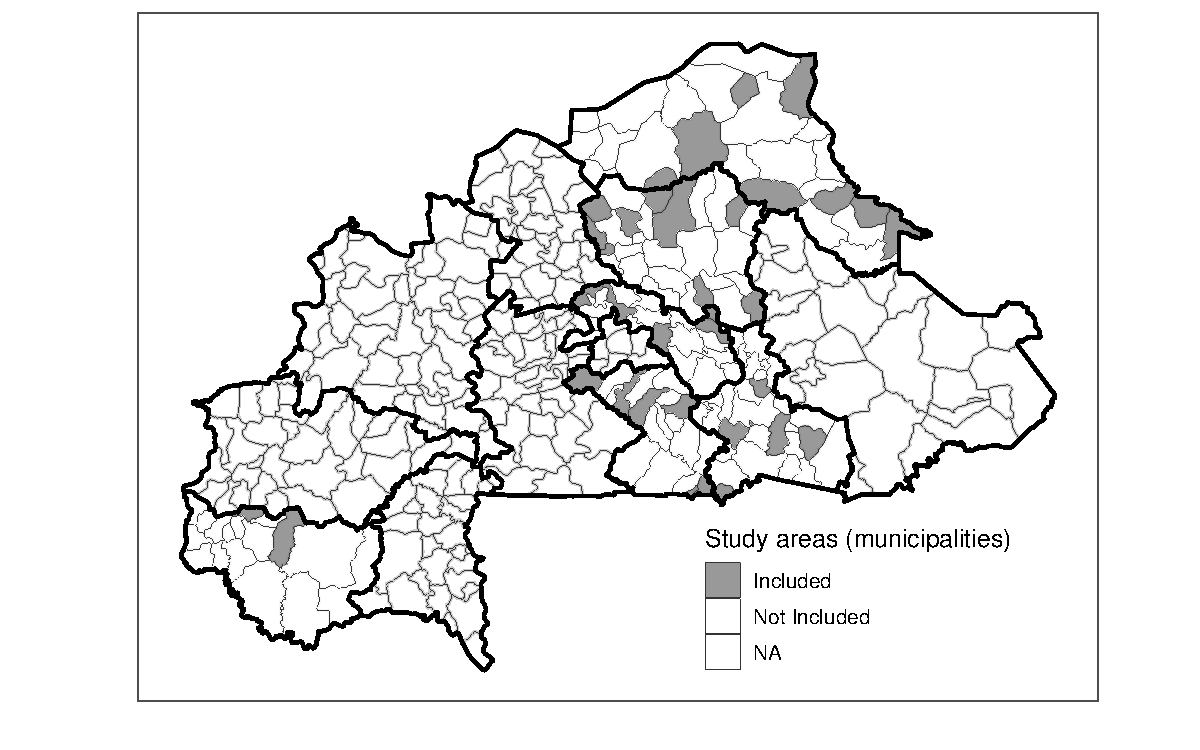
\includegraphics[width=\textwidth]{Figures/BF_StudyAreas.pdf}
\end{center}
\caption{Study areas. }
\label{FigMap}
\end{figure}

\begin{figure}
\vspace{1em}

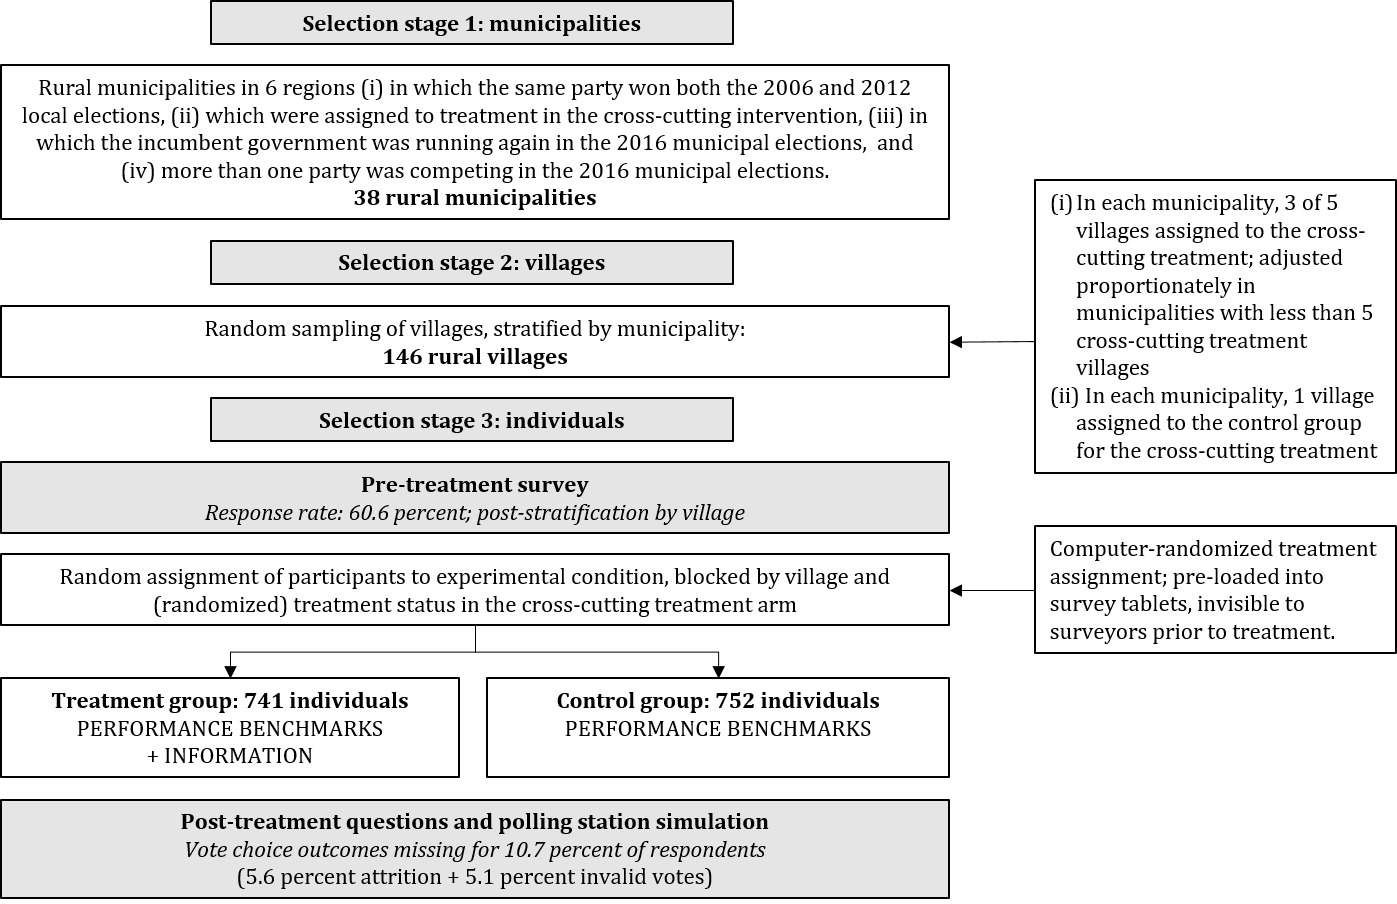
\includegraphics[width=\textwidth]{Figures/BF_ConsortDiagram.png}

\caption{Treatment assignment and selection of study population. Note: Attrition in vote choice outcomes is largely due to the chemical decomposition of ballot identifiers that were printed in UV-visible ink and accidentally exposed to sunlight. }
\label{FigConsortDiagram}
\end{figure}

\subsection{Defining ``good'' and ``bad'' news}
	
Using the common notation of the studies in this volume, we define the information content $Q$ as the quantile of the distribution of municipal service delivery performance scores within a region to which the incumbent municipal government's performance corresponds, i.e. $Q=1$ if the incumbent government was the top-performer in the region and $Q=0.5$ if the incumbent was the median performer. To elicit study participants' prior beliefs $P$, study participants were given the total number of municipalities in their region and were asked to guess their municipal government's rank among those $M$ municipalities, which was then divided by $M$ to yield quantiles. So both $P$ and $Q$ are greater than zero and less than or equal to one. 

We define the ``good news'' subgroup as the subset of study participants for whom either $P-Q<0$ or both $P-Q=0$ and $Q\geq0.5$, i.e. the study participants who underestimated their municipal government's performance rank, plus the study participants who correctly estimated their municipal government's performance rank and their municipal government's performance was greater than or equal to the median in their region. Analogously, we define the ``bad news'' subgroup as those study participants for whom either $P-Q>0$ or both $P-Q=0$ and $Q<0.5$. By this definition, the information treatment was ``good news'' for study participants who previously underestimated their incumbent municipal government's relative performance (in comparison to other municipalities of their region) and ``bad news'' for those who previously overestimated it. 

\section{Effects of Performance Information}

Like the other studies in this volume, we estimate the effects of our experimental treatment -- access to performance information -- separately for two subgroups: Those study participants who had underestimated incumbent performance at baseline (the ``good news'' subgroup) and those who had overestimated incumbent performance (the ``bad news'' subgroup). Our analyses focus on two outcomes of interest: vote choice and turnout intent. We first explain how data on these individual-level outcomes was collected. We then report average treatment effects for each of the two subgroups, before presenting results on treatment effect heterogeneity. 
 
\subsection{Data and measurement}

Data on intended vote choice and intent to vote was collected immediately following the information treatment, by our implementation partner Innovations for Poverty Action (IPA) in April and May 2016, prior to the May 22 municipal elections. The outcome data was collected by the same surveyors who carried out the baseline survey and administered the treatment and control conditions. 

%Prior to the information and control treatments, baseline data was recorded on individual characteristics, knowledge and attitudes with respect to municipal elections and politics, including whether the respondent voted in the 2012 municipal elections and whether he or she supported the incumbent party. In the control condition, was then delivered to all study participants, after which they were asked for their beliefs regarding the performance of the previous incumbent municipal government. Subsequently, the performance information treatment was delivered to members of the treatment group. Finally, we collect data on the post-treatment outcomes of interest.

\emph{Intended vote choice}

Study participants' intended vote choice was measured through a polling station simulation, immediately following the information treatment. This approach was chosen in order to minimize respondent-related measurement biases. Since vote choice is a potentially sensitive question, respondents may be reluctant to reveal information if they are asked directly, even if they are told that their responses will be kept confidential. Also, self-reported vote choice may be subject to social desirability bias. Respondents' answers could be influenced, consciously or subconsciously, by what they perceive to the most socially accepted choice or the surveyor's preference. This makes it necessary to measure vote choice under conditions of complete anonymity and in a situation that resembles the actual elections as much as possible. 

We asked study participants to participate in a pre-election poll, where they would cast a vote in a mock polling station, complete with voting booths and sealed ballot boxes. The layout of the ballots in the polling station simulation was identical to those that were subsequently used in the actual elections. Study participants were informed this was not the real election, and that our objective was to estimate the number of votes different parties will get in the actual elections on May 22. They were also informed that aggregate results of the mock election would eventually be publicly accessible on the internet, so that people could compare them with the official election results. Respondents were furthermore informed that their vote would be completely confidential and that no one, including no government authority, would be able to infer from our data who the respondent voted for in the mock election. 

To ensure anonymity of the votes cast in the mock election, each ballot contained two unique ID codes. One was printed on a detachable receipt at the top of the ballot. Prior to handing the ballot to the respondent, the surveyors detached this portion of the ballot and explained to respondents that they are sending it back to their organization as proof of the number of votes cast, which would be cross-checked against the number of unused ballots that were returned. This procedure closely mirrors the use of unique, detachable ballot receipts in the actual municipal elections. The second ID was printed in invisible ultraviolet ink directly on the main part of the ballot. The two ID codes were linked through a concordance list that was locked in advance of data collection. The surveyors recorded only the visible ID from the detached receipts together with the survey data. The surveyors were not aware of the invisible ink identifiers that were printed on the ballots. 

Ballots that were submitted in the mock election were handled strictly separately from the survey data. Vote choices were manually entered by a separate vote count team, along with the invisible ballot identifier codes that were inspected under ultraviolet light. Our data collection partner did not have access to the concordance list that would have allowed them to match ballot data to individual survey responses. Instead, our data collection partner provided us with anonymized survey data that contained the visible ballot identifiers, as well as with the voting data that contained the invisible identifiers. Using the concordance list, we matched the identifiers from the ballots to the identifiers in the survey data \emph{after anonymization} of the survey data. That way, we were able to ensure full anonymity of study participants' vote choices, because we had no access to personal identifying information in the survey, whereas our data collection partner, who had access to respondents' identifying information, did not have access to the concordance list by which it could be matched to individuals' vote choices.

\emph{Turnout intent}

We use a self-reported measure of turnout intent, based on the following survey question: ``Considering that in the real elections citizens have a choice whether to vote or abstain, how likely is it that you will actually vote in the municipal elections on May 22nd?" Response options for this question are: (i) I definitely plan to vote and will make every reasonable effort to do so; (ii) I will probably vote, but am not completely sure yet; (iii) I am not sure yet, but I tend towards voting; (iv) I am not sure yet, but I tend towards not voting; (v) I probably won't vote, but am not completely sure yet; and (vi) I am determined not to vote, and I will try hard to avoid it. For ease of analysis, we assume that the six response categories approximately map into turnout probabilities of 0, 0.2, 0.4, 0.6, 0.8, and 1.

\subsection{Effects on vote choice and intent to vote}

The average added effect of access to performance information on pro-incumbent voting in the polling station simulation is statistically indistiguishable from zero. In the overall sample, the estimated 95 percent confidence interval ranges from -1.7 percentage points to +8.0 percentage points. 

In the ``good news'' subgroup, i.e. among voters who underestimate incumbent performance, our population-weighted estimate of is that 34.1 percent intended to vote for the incumbent party, based on the vote choices in the control group. Performance information changed the pro-incumbent voting intent between -11.5 and +7.6 percentage points (95 percent CI). We find no evidence that study participants who had underestimated the incumbent's performance more severely reacted more strongly to the information treatment. 

In the ``bad news'' subgroup, i.e. among voters who overestimated incumbent performance, our population-weighted estimate is that 29.4 percent intended to vote for the incumbent party, while the information treatment changed pro-incumbent voting intent between -0.3 and +11.5 percentage points (95 percent CI). Again, we find no evidence that study participants who had overestimated the incumbent's performance more severely reacted more strongly to the information treatment. 

With respect to self-reported turnout propensity, access to performance information has no substantially significant effect in either subgroup. We find no evidence that receiving better-than-expected news about incumbent performance increases voter turnout among those who had underestimated the incumbent's performance or that worse-than-expected information would suppress voter turnout among those who had overestimated the incumbent's performance.  

If we combine voting intent and self-reported turnout propensity to calculate expected effects on the incumbent's ultimate vote share, access to performance information increased the incumbent's vote share in the ``bad news'' subgroup, by an estimated 5.8 percentage points (s.e. 3.0 percentage points). In the ``good news'' subgroup, it is more likely that information access decreased, rather than increased, the incumbent vote share (point estimate -4.4 percentage points, s.e. 4.9 percentage points). 

In interpreting these results, it is important to keep in mind that they reflect only the added causal impact of truthful information content, after providing voters with a detailed explanation of municipal government responsibilities and benchmarks for their performance. In the eventual municipal elections, 29.4 percent of voters from the same set of villages voted for the local incumbent, whereas the corresponding estimate from the polling station simulation is 30.8 percent ($\pm$3.5 percentage points) in the control group. The difference is minimal and insignificant. That being said, it remains possible that an effect of information about the municipal service delivery indicators and performance benchmarks on pro-incumbent voting was obscured by the time gap of up to a few weeks between our survey and the actual elections. 

\begin{table}

    \begin{center}
    \begin{tabular}{l c c c }
    \hline
    &(1)&(2)&(3)\\
    &Pro-incumbent&Turnout &Extrapolated incumbent\\
    &voting intent& Propensity&vote share\\
    \hline
    \textbf{Panel A: Pooled}\\
    \hline
    Information treatment&0.035&0.019&0.029\\
    &(0.024)&(0.013)&(0.025)\\
    $\times$ Gap between priors and information$^{(s)}$ &0.027&0.0069&0.03\\
    &(0.025)&(0.013)&(0.025)\\
    Observations&1333&1487&1316\\
    \hline
    \textbf{Panel B: Good News Subgroup}\\
    \hline
    Information treatment&-0.018&0.0045&-0.041\\
    &(0.049)&(0.025)&(0.05)\\
    $\times$ Gap between priors and information$^{(s)}$ &0.025&-0.0062&0.029\\
    &(0.05)&(0.025)&(0.05)\\
    Observations&421&477&417\\
    \hline
    \textbf{Panel C: Bad News Subgroup}\\
    \hline
    Information treatment&0.051$^{*}$&0.023&0.055$^{*}$\\
    &(0.03)&(0.016)&(0.03)\\
    $\times$ Gap between priors and information$^{(s)}$ &0.0091&0.011&-0.0045\\
    &(0.031)&(0.016)&(0.032)\\
    Observations&912&1010&899\\
    \hline\hline
    \end{tabular}
    \end{center}

\caption{Average treatment effects and interaction with the gap between prior beliefs and performance information ($P-Q$). The table shows OLS coefficients. All specifications include village fixed effects. Standard errors in parentheses. $^{(s)}$ Mean-centered/ standardized within subgroup. $^{*} p<0.1$, $^{**} p<0.05$, $^{***} p<0.01$. }
\end{table}

\subsection{Heterogeneous treatment effects}

In line with the common analysis plan, we further examined if the effects of performance information on vote choice and voter turnout varied with relevant individual- and village-level covariates. In Tables \ref{TableHeterogeneity1} and \ref{TableHeterogeneity2}, we report the estimated linear interaction coefficients between the information treatment and (1) whether a respondent report to have voted for the incumbent in 2012, (2) whether s/he expects to receive a campaign gift (by any party), (3) perceived electoral competitiveness at the village level, measured by voters expectations about the incumbent's vote margin over the strongest local opposition party (averaged among the respondents in the control group in a given village), and (4) respondents' perceptions of electoral integrity, specifically of the chance that the counting of votes will be fair and of the risk that ballots are not secret. 

Of these, only perceived local competitiveness shows a significant interaction effect with the information treatment, and only in the ``good news'' subgroup, where its effect on pro-incumbent voting is particularly negative in villages where the incumbent ties with the opposition. 
%\begin{itemize}
%\item [H7] Information effects are more positive for voters with weaker partisan identities. 
%\item [H8] Information effects are more positive for voters who have not received clientelistic benefits from any candidate
%\item [H10] Informational effects are stronger in more competitive elections. 
%\item [H11] Informational effects are stronger in settings in which elections are believed to be free and
%fair.
%\end{itemize}

\begin{table}

    \begin{center}
    \begin{tabular}{l c c c c c c }
    \hline
    &\multicolumn{6}{c}{\emph{Pro-Incumbent Voting Intent}}\\
    &(1)&(2)&(3)&(4)&(5)&(6)\\
    \hline
    \textbf{Panel A: Pooled}\\
    \hline
    Information treatment &0.035&0.061$^{*}$&0.02&0.015&0.016&0.035\\
    &(0.024)&(0.037)&(0.027)&(0.037)&(0.028)&(0.025)\\
    $\times$ Incumbent supporter & &-0.047& & & & \\
    & &(0.051)& & & & \\
    $\times$ Expects campaign gift & & &0.083 & & & \\
    & & &(0.065) & & & \\
    $\times$ abs(Expected vote margin) & & & &0.11& & \\
    & & & &(0.12$^{(c)}$)& & \\
    $\times$ Fair vote count$^{(s)}$ & & & & &-0.0028& \\
    & & & & &(0.029)& \\
    $\times$ Ballot secrecy$^{(s)}$ & & & & & &-0.011\\
    & & & & & &(0.026)\\
    Observations &1333&1333&1333&1333&1056&1315\\
    \hline
    \textbf{Panel B: Good News Subgroup}\\
    \hline
    Information treatment &-0.019&-0.0097&-0.049&-0.12$^{*}$&-0.033&-0.019\\
    &(0.049)&(0.072)&(0.054)&(0.068)&(0.061)&(0.049)\\
    $\times$ Incumbent supporter & &-0.014& & & & \\
    & &(0.1)& & & & \\
    $\times$ Expects campaign gift & & &0.15 & & & \\
    & & &(0.12) & & & \\
    $\times$ abs(Expected vote margin) & & & &0.46$^{*}$& & \\
    & & & &(0.24$^{(c)}$)& & \\
    $\times$ Fair vote count$^{(s)}$ & & & & &-0.048& \\
    & & & & &(0.063)& \\
    $\times$ Ballot secrecy$^{(s)}$ & & & & & &-0.061\\
    & & & & & &(0.049)\\
    Observations &421&421&421&421&310&419\\
    \hline
    \textbf{Panel C: Bad News Subgroup}\\
    \hline
    Information treatment &0.052$^{*}$&0.069&0.031&0.081$^{*}$&0.023&0.051$^{*}$\\
    &(0.03)&(0.046)&(0.034)&(0.046)&(0.034)&(0.031)\\
    $\times$ Incumbent supporter & &-0.028& & & & \\
    & &(0.063)& & & & \\
    $\times$ Expects campaign gift & & &0.12 & & & \\
    & & &(0.082) & & & \\
    $\times$ abs(Expected vote margin)  & & & &-0.069& & \\
    & & & &(0.17$^{(c)}$)& & \\
    $\times$ Fair vote count$^{(s)}$ & & & & &0.029& \\
    & & & & &(0.036)& \\
    $\times$ Ballot secrecy$^{(s)}$ & & & & & &-0.003\\
    & & & & & &(0.033)\\
    Observations &912&912&912&912&746&896\\
    \hline\hline
    \end{tabular}
    \end{center}

\caption{Heterogeneous treatment effects. The dependent variables is pro-incumbent voting in the polling station simulation. The table reports OLS coefficients. All specifications except (4) include village fixed effects. Standard errors in parentheses. $^{(c)}$Adjusted for clustering at the village level. $^{(s)}$Mean-centered/standardized within subgroup. $^{*} p<0.1$, $^{**} p<0.05$, $^{***} p<0.01$. }
\label{TableHeterogeneity1}
\end{table}


\begin{table}

    \begin{center}
    \begin{tabular}{l c c c c c c }
    \hline
    &\multicolumn{6}{c}{\emph{Extrapolated Incumbent Vote Share}}\\
    &(1)&(2)&(3)&(4)&(5)&(6)\\
    \hline
    \textbf{Panel A: Pooled}\\
    \hline
    Information treatment &0.029&0.042&0.013&0.0044&0.0092&0.029\\
    &(0.025)&(0.039)&(0.028)&(0.037)&(0.028)&(0.025)\\
    $\times$ Incumbent supporter & &-0.021& & & & \\
    & &(0.052)& & & & \\
    $\times$ Expects campaign gift & & &0.086 & & & \\
    & & &(0.066) & & & \\
    $\times$ abs(Expected vote margin) & & & &0.12& & \\
    & & & &(0.12$^{(c)}$)& & \\
    $\times$ Fair vote count$^{(s)}$ & & & & &-0.0073& \\
    & & & & &(0.03)& \\
    $\times$ Ballot secrecy$^{(s)}$ & & & & & &0.0032\\
    & & & & & &(0.026)\\
    Observations &1316&1316&1316&1333&1040&1298\\
    \hline
    \textbf{Panel B: Good News Subgroup}\\
    \hline
    Information treatment &-0.044&-0.071&-0.081&-0.14$^{**}$&-0.056&-0.044\\
    &(0.049)&(0.076)&(0.055)&(0.068)&(0.061)&(0.049)\\
    $\times$ Incumbent supporter & &0.052& & & & \\
    & &(0.1)& & & & \\
    $\times$ Expects campaign gift & & &0.18 & & & \\
    & & &(0.12) & & & \\
    $\times$ abs(Expected vote margin) & & & &0.5$^{**}$& & \\
    & & & &(0.24$^{(c)}$)& & \\
    $\times$ Fair vote count$^{(s)}$ & & & & &-0.081& \\
    & & & & &(0.065)& \\
    $\times$ Ballot secrecy$^{(s)}$ & & & & & &-0.031\\
    & & & & & &(0.049)\\
    Observations &417&417&417&421&306&415\\
    \hline
    \textbf{Panel C: Bad News Subgroup}\\
    \hline
    Information treatment &0.055$^{*}$&0.063&0.036&0.078$^{*}$&0.026&0.054$^{*}$\\
    &(0.03)&(0.048)&(0.034)&(0.047)&(0.034)&(0.031)\\
    $\times$ Incumbent supporter & &-0.0084& & & & \\
    & &(0.064)& & & & \\
    $\times$ Expects campaign gift & & &0.11 & & & \\
    & & &(0.083) & & & \\
    $\times$ abs(Expected vote margin)  & & & &-0.081& & \\
    & & & &(0.17$^{(c)}$)& & \\
    $\times$ Fair vote count$^{(s)}$ & & & & &0.032& \\
    & & & & &(0.036)& \\
    $\times$ Ballot secrecy$^{(s)}$ & & & & & &0.0045\\
    & & & & & &(0.033)\\
    Observations &899&899&899&912&734&883\\
    \hline\hline
    \end{tabular}
    \end{center}

\caption{Heterogeneous treatment effects. The dependent variable is pro-incumbent voting, adjusted for self-reported turnout intent. The table reports OLS coefficients. All specifications except (4) include village fixed effects. Standard errors in parentheses. $^{(c)}$Adjusted for clustering at the village level. $^{(s)}$Mean-centered/standardized within subgroup. $^{*} p<0.1$, $^{**} p<0.05$, $^{***} p<0.01$. }
\label{TableHeterogeneity2}
\end{table}

\section{Cross-Cutting Experiment: Personal Exposure to Municipal Governance Processes}

In addition to the common treatment arm -- providing voters with information about incumbent performance -- we carried out a cross-cutting experimental treatment with a random subset of our study participants, prior to the information experiment. This cross-cutting treatment consisted of personalized invitations to volunteer as ``citizen observers'' at a meeting of the municipality's special delegation. With the support of our government partner and six regional NGOs, we convinced the presidents of the special delegations (the interim mayors) to personally invite randomly sampled voting-age residents of the municipality to a special delegation meeting. The invited citizens received a formal invitation letter (addressed by name and hand-signed by the president of the special delegation) that encouraged them to attend a specific special delegation meeting as ``citizen observer'' and to share their views in a question and answer session that would follow the meeting. Records collected at the meetings show that more than 60 percent of the invited citizens actually attended. 

Our goal in evaluating this cross-cutting treatment is to test if personal experience with municipal decision processes influences voters' interest in and response to performance information. The fact that the elected municipal councils were temporarily suspended and replaced by externally appointed special delegations created a unique opportunity to shed light on this question. It means that we could expose voters to the municipal governance process without simultaneously exposing them to the incumbent and thus inevitably affecting their level of information about incumbent performance. 

In addition to evaluating the effects of the ``citizen observer'' intervention on civic participation more generally (in a larger field experiment in 118 rural municipalities \citep{CitizenObserverPAP} of which the 38 municipalities covered by this study are a subset), we also pre-specified three hypotheses about its interaction with the information treatment.\footnote{Hypotheses 3.1, 3.2a and 3.2b in our analysis plan.} Specifically, we intend to test if having been selected as a ``citizen observer''
\begin{enumerate}
\item increases citizens' interest in performance information and the attention they pay to it, 
\item causes voters to place greater weight on expected performance in evaluating electoral candidates, 
\item and as a result of the two aforementioned mechanisms reinforces the effect of performance information on vote choice. 
\end{enumerate}

In other words, we are interested in whether personal experiences with municipal governance processes makes voting in municipal elections more ``performance-based'', as opposed to ``affinity based'' (i.e. driven by sources of political affinity that are unrelated to the a party's expected performance in governing the municipality, such as clientelism, ideology, identity politics, or national-level politics). Receiving an invitation to serve as citizen observer and subsequently attending a special delegation meeting could cause citizens to reflect about the importance of municipal government performance for their own lives, but also cause them to associate questions of municipal governance with a positive, memorable experience. Therefore, we expect that individuals in the cross-cutting treatment arm will show increased interest in performance information and greater concern for municipal government performance, relative to the control group. However, since our experiment shows that a positive reception of the information treatment and strong self-reported concern for municipal service delivery performance did not translate into the expected results, we are forced to reconsider whether we expect that the cross-cutting treatment reinforces the impact of performance information on vote choice, or rather attenuates or reverses it.  

\section{Conclusion}

In examining the effects of performance information about incumbent municipal governments in Burkina Faso, our experiment focused on isolating the effects of information content from other aspects of political information interventions. The results were unexpected, at least in light of the theoretical expectations that were articulated in the meta-analysis plan \citep{MetaPAP}. Rather than shifting voters' support for the incumbent in the direction of the information signal, information access appeared to do the opposite. Voters who had previously overestimated incumbent performance were approximately six percentage points more likely to support the incumbent after receiving ``bad news'' about the incumbent government. This was not the case among voters who had previously underestimated incumbent performance, where we find that ``good news'' had no significant effect (and our point estimates are negative). Overall, we observe that information access seemed to benefit the electoral prospects of poorly performing incumbents without helping high-performing incumbents. At first glance, this pattern of results, although estimated with considerable noise, seems at odds with conventional thinking about retrospective electoral accountability. 

However, amidst the other experiments in this volume, our results are not an outlier. The signs of subgroup-specific treatment effects in our experiment are the same as in Arias et al. (this volume) and Adida et al. (this volume; in the case of actual election results, rather than self-reported vote choice). They contrast with the ``Meet the Candidate'' experiment in Uganda, where those voters who received better-than-expected information about a candidate where more likely to vote for that candidate (Izama Platas and Raffler, this volume), and Buntaine et al. (this volume), where voters who received worse-than-expected information about local budget discrepancies were less likely to vote for the incumbent district councilors. 

What might explain the counterintuitive effects we observe? In our first attempt at understanding this result we relied on a detailed analysis strategy we had developed without prior knowledge of the results: A full results-blind report that focused on seven important questions along the causal chain that connects study participants' processing of performance information with their ultimate voting behavior. 

A first important observation was that the distribution of prior beliefs cannot explain why low-performing incumbents gained from information dissemination. Unlike \citep{Arias2017}, who conjecture that incumbents gained from information about fiscal malfeasance, because voters had originally expected even greater malfeasance, our results-blind analysis revealed that voters in rural Burkina Faso were biased towards \emph{overestimating} incumbent performance. In fact, low-performing incumbents were particularly likely to be overestimated, but disclosing performance information did not reduce their electoral support. 

We next turned to how voters who overestimated incumbent performance might differ from those who underestimated incumbent performance. For example, \citep{Adida2017} hypothesize that motivated reasoning explains why negative performance information failed to reduce politicians' electoral support among co-ethnic voters. If some voters selectively ignore negative information about the incumbent, they are likely to be biased towards overestimating incumbent performance. Those voters are more likely to be in the ``bad news'' subgroup, whereas voters who process information more rationally would be equally likely to be in the ``bad news'' or ``good news'' subgroup, provided that they had prior access to unbiased information. As we argued in our results-blind report, these selection effects could lead to the counterintuitive outcome that information which is ``bad news'' for most voters leads to a more positive average assessment of the incumbent, simply because the beliefs of voters who underestimated incumbent performance are corrected more easily than the beliefs of voters who overestimated incumbent performance. 

However, we find no support for this motivated reasoning mechanism in our data. Instead, it appears that information about the incumbent government's past performance had generally no significant impact on expectations about future performance, in either subgroup. Interestingly though, receiving good news about the incumbent government appeared to have negative externalities on study participants' expectations about the \emph{electoral challengers}. Such externalities, however, cannot explain why performance information \emph{failed} to increase incumbent support in the ``good news'' subgroup. Moreover, if information about past performance failed to significantly change expectations about future performance, why did the information treatment nevertheless increase incumbent support in the ``bad news'' subgroup? 

Having found no support for either of these potential mechanisms, we turned our attention to a new explanation that had hitherto been neglected in the literature on information and voting behavior: The fact that voters might be ambiguity averse and therefore prefer those candidates about whom they have the most information. In \citep{LierlHolmlundAmbiguity}, we argue that one-sided performance information about the incumbent reduces ambiguity about that candidate, turning unknown risks about incumbent performance into known risks. If voters have a strong preference for known risks over unknown risks, even bad news about incumbent performance could make the incumbent the more attractive choice. 

Our data strongly support this interpretation (Table \ref{TableAmbiguity}), suggesting that the impact of performance information is moderated by voters' uncertainty about their prior beliefs. The more uncertain voters were about the incumbent's performance, the more did the information treatment cause them to support the incumbent, conditional on the incumbent's actual incumbent performance. As it happened, voters who overestimated incumbent performance were much more uncertain about their assessment than voters who underestimated incumbent performance (Figure \ref{FigBiasCertainty}). If voters are ambiguity averse, this correlation between prior beliefs and uncertainty, whatever may be the cause of it, can plausibly explain why voters who received ``bad news'' about the incumbent were more likely to vote for the incumbent: Given voters' uncertainty, the ambiguity-reducing effect of information access may have been strong enough to outweigh the fact that receiving ``bad news'' about incumbent performance reduces the attractiveness of the incumbent party.  

\begin{table}

    \begin{center}
    \begin{tabular}{l c c c}
    \hline
    &\multicolumn{3}{c}{\emph{Pro-incumbent vote choice}}\\
    &(1)&(2)&(3)\\
    \hline  
    Information treatment&-0.037&-0.037&-0.042\\
    &(0.035)&(0.035)&(0.035)\\
    Uncertainty about priors&-0.035&-0.0043&-0.048\\
    &(0.058)&(0.059)&(0.059)\\
    Information treatment$\times$Uncertainty&0.22$^{***}$&0.22$^{***}$&0.23$^{***}$\\
    &(0.078)&(0.077)&(0.077)\\
    Incumbent performance$^{(s)}$&&-0.45&-0.5\\
    &&(1.2)&(1.2)\\
    Prior beliefs$^{(s)}$&&-0.0015&0.00027\\
    &&(0.014)&(0.014)\\
    Voted for Incumbent in 2012&&0.11&0.092\\
    &&(0.026)&(0.027)\\
    Individual controls&&&Yes\\
    Village \& municipality fixed effects&Yes&Yes&Yes\\
    \hline
    Observations&1333&1333&1333\\
    \hline\hline
    \end{tabular}
    \end{center}
    \caption{Heterogeneous effects of performance information by uncertainty about prior beliefs. Uncertainty is measured on a 5-point scale (0...completely certain to 1...no idea). The table reports OLS coefficients. Standard errors in parentheses. Individual controls in column (3) are gender, age, years of education. $^{(s)}$Standardized. $^{*} p<0.1$ $^{**} p<0.05$ $^{***} p<0.01$. }
    

\label{TableAmbiguity}
\end{table}

\begin{figure}
\begin{center}
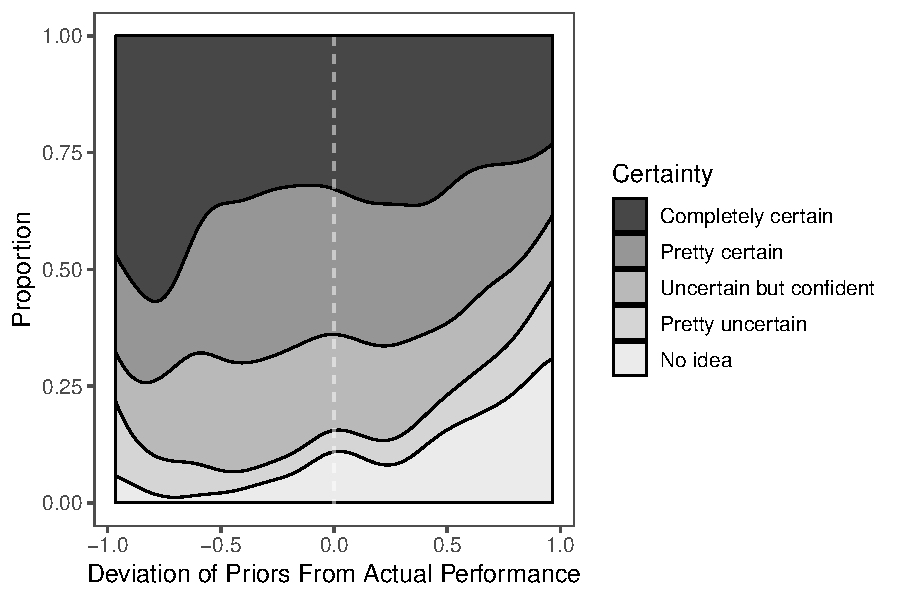
\includegraphics[width=0.8\textwidth]{./Figures/BF_FigBiasCertainty.pdf}
\end{center}
\caption{Voters who overestimate incumbent performance are less certain about their beliefs. } 
\label{FigBiasCertainty}
\end{figure}

\label{sec:References}
\bibliographystyle{apalike}
\bibliography{./Bibliography/BF_bibliography}

\end{document}